\documentclass[tikz, border=10pt]{standalone}
\usetikzlibrary{calc, automata, chains, arrows.meta}
\begin{document}
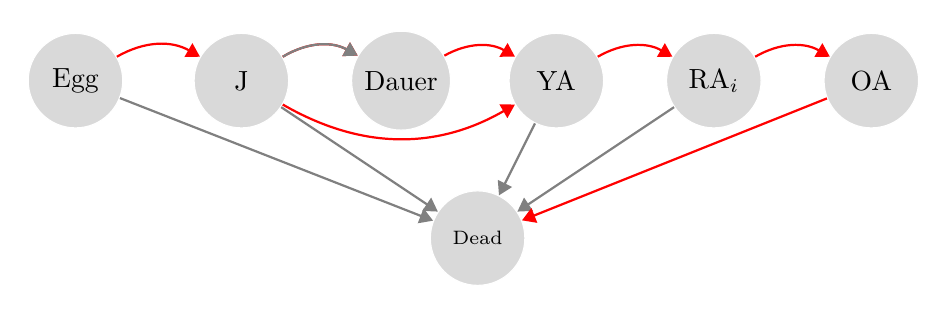
\begin{tikzpicture}[start chain = going right,
  -Triangle, every loop/.append style = {-Triangle}]
   \node[state, minimum size=0.cm, draw=white]  at (0.2, 0.4) (9) {};
   \node[state, minimum size=0.cm, draw=white]  at (8, 0.5) (10) {};
    \node[state, on chain, minimum size=1.2cm, fill=gray!30, draw=white]  at (0, 0) (0) {Egg};
    \node[state, on chain, minimum size=1.2cm, fill=gray!30, draw=white] at (0.5, 0) (1) {J};
    \node[state, on chain, minimum size=1.2cm, fill=gray!30, draw=white] at (2.5, 0)  (2) {Dauer};
    \node[state, on chain, minimum size=1.2cm, fill=gray!30, draw=white]  at (4.5, 0) (3) {YA};
    \node[state, on chain, minimum size=1.2cm, fill=gray!30, draw=white] at (6.5, 0)  (4) {RA$_i$};
    \node[state, on chain, minimum size=1.2cm, fill=gray!30, draw=white] at (8.5, 0)  (5) {OA};

    \node[state, on chain, minimum size=1.2cm, fill=gray!30, draw=white] at (3.5, -2)  (6) {\scriptsize Dead};
 
  %\draw (10) edge[dotted, bend right, thick, black] (9);
  \foreach \i in {0,...,1} {
    \draw let \n1 = { int(\i+1) } in
      (\i)  edge[bend left, thick, red] (\n1);
  }

  \foreach \i in {3,...,4} {
    \draw let \n1 = { int(\i+1) } in
      (\i)  edge[bend left, thick, red] (\n1);
  }

  \draw    (1)  edge[bend left, thick, gray]  (2);
  \draw    (1)  edge[bend right, thick, red]  (3);
  \draw    (2)  edge[bend left, thick, red]  (3);

  \draw    (0)  edge[thick, gray]  (6);
  \draw    (1)  edge[thick, gray]  (6);
  \draw    (3)  edge[thick, gray]  (6);
  \draw    (4)  edge[thick, gray]  (6);
  \draw    (5)  edge[thick, red]  (6);
  
\end{tikzpicture}
\end{document}